\documentclass[12pt,letterpaper]{article}
\usepackage{pgf, tikz}
\usetikzlibrary{arrows, automata}

\begin{document}

    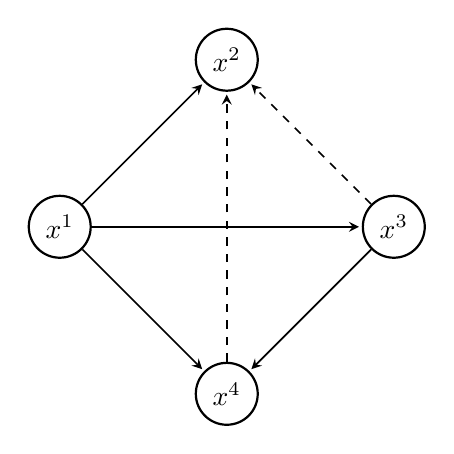
\begin{tikzpicture}[
            > = stealth, % arrow head style
            shorten > = 1pt, % don't touch arrow head to node
            auto,
            node distance = 3cm, % distance between nodes
            semithick % line style
        ]

        \tikzstyle{every state}=[
            draw = black,
            thick,
            fill = white,
            minimum size = 4mm
        ]

        \node[state] (x1) {$x^1$};
        \node[state] (x2) [above right of=x1] {$x^2$};
        \node[state] (x3) [below right of=x2] {$x^3$};
        \node[state] (x4) [below right of=x1] {$x^4$};

        \path[->] (x1) edge node {} (x2);
        \path[->] (x1) edge node {} (x3);
        \path[->] (x1) edge node {} (x4);
        \path[->] (x3) edge node {} (x4);
        \path[->,dashed] (x3) edge node {} (x2);
        \path[->,dashed] (x4) edge node {} (x2);
    \end{tikzpicture}

\end{document}